%!TEX root = Thesis.tex
\chapter{Concept}
     The chapter poses and describes a concept of a user-friendly generic frontend for exploring sensor data, 
     through designing a software architecture and a mockup of a web-based user interface that in the same time controlled and provisioned by end users request. The concept is developed based on the analysis of the current state of the art, up-to-date technologies and usability characteristics. According to defined requirements in chapter 2 to the third-party services and applications and knowledges gained from the studied related works (chapter 3), was proposed concept based on 3-tier architecture and in details described in section 4.2 - 4.4.

\section{3-tier Architecture}
Since the concept of a generic frontend should be distributed as much as possible, it is necessary to determine software architecture 
to a 3-tier architecture, in which presentation, application processing, and data management functions are logically separated.
Figure 4.1 shows this architecure:
\begin{itemize}
\item Data Tier: data from different types of sensors
\item Application Tier: registry and proxy
\item Client Tier: web-based UI
\end{itemize} 
\begin{figure}[!ht]
\centering
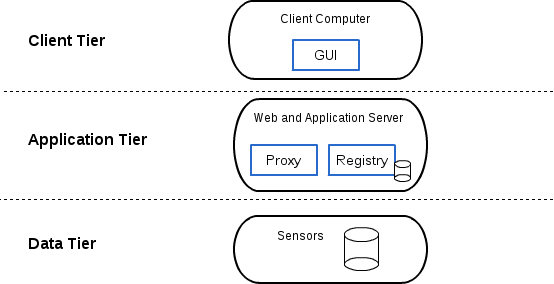
\includegraphics[scale=0.7]{images/3tier.png}   
\caption[3-tier Architecture]{3-tier Architecture}
\label{img:3-tier Architecture}                           
\end{figure}
\emph{Client Tier} hosts the presentation layer components. The main function of the interface is to translate tasks and results to graphical user interface that can be easily understandable and explorable from any kind of device. That satisfy requirements of the usability(section 3.4).
\newline
\emph{Application Tier} includes business logic, logic tier, data access tier. It controls an application's functionality by performing detailed processing, transformation of one type data to another one, defines an interface of interconnection between client tier and data tier.
\newline
\emph{Data Tier} consists source of data that have to be retrieved by application tier to a Client Tier, by request from a end user. This tier keeps data neutral and independent from application server or business logic. Giving data its own tier also improves scalability. 
\newline
The three tiers architecture may seem similar to the model-view-controller (MVC) concept. However, topologically they are different. A fundamental rule in a three tier architecture is the client tier never communicates directly with the data tier; in a three-tier model all communication must pass through the middle tier. Conceptually the three-tier architecture is linear. However, the MVC architecture is triangular: the view sends updates to the controller, the controller updates the model, and the view gets updated directly from the model.
From a historical perspective the three-tier architecture concept emerged in the 1990s from observations of distributed systems (e.g., web applications) where the client, middleware and data tiers ran on physically separate platforms. Today, MVC and similar model-view-presenter (MVP) are Separation of Concerns design patterns that apply exclusively to the presentation layer of a larger system. In simple scenarios MVC may represent the primary design of a system, reaching directly into the database; however, in most scenarios the Controller and Model in MVC have a loose dependency on either a Service or Data layer/tier. This is all about Client-Server architecture.

In the next chapter begins detailed explaination about every tier in 3-tier architecture.

\section{Client Tier}

\begin{figure}[!ht]
\centering
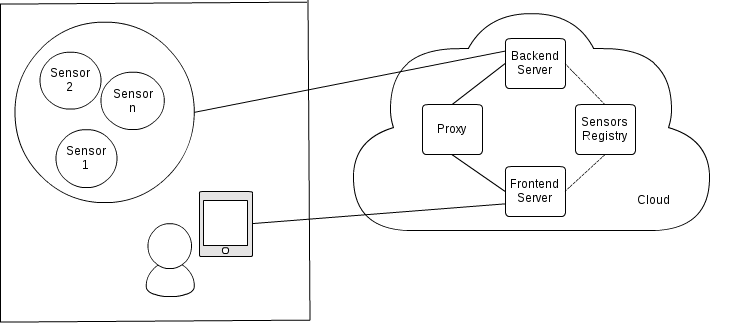
\includegraphics[scale=0.5]{images/User_Case.png}   
\caption[Use Case]{Use Case}
\label{img:structure}                           
\end{figure}
  \subsection{GUI}
  \begin{figure}[!ht]
  \centering
  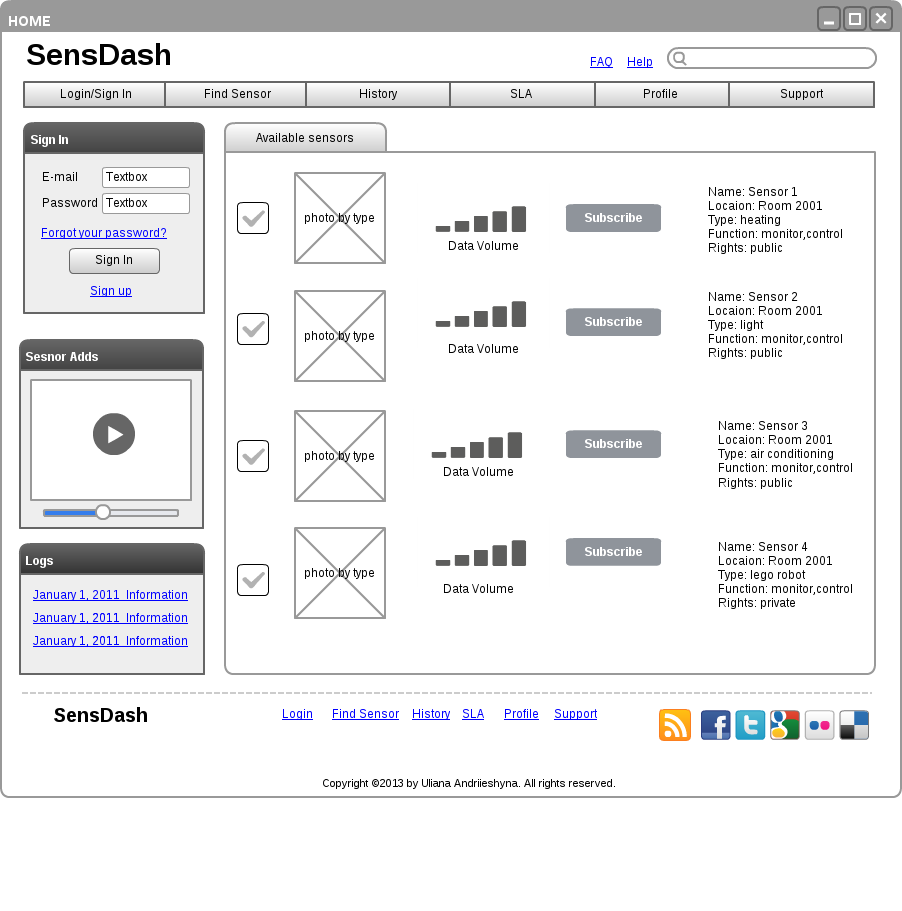
\includegraphics[scale=0.5]{images/Mockup.png}   
  \caption[GUI Mocku]{GUI Mockup}
  \label{img:GUI Mockup}                           
  \end{figure}
  1. Sensor icon defines what is the current type of sensor, e.g. light, temperature, heating, robot lego, etc.
  2. User can subscribe only to the available services. If some services become unavailable they will be automaticaly inactivated and after refreshing will be deleted from the list.
  3. Data Volume shows what is the average data stream volume needed to retrieve sensor data(Kb/s).

\section{Application Tier}
- Web server
\newline
- Registry
\newline
- Proxy

\begin{figure}[!ht]
\centering
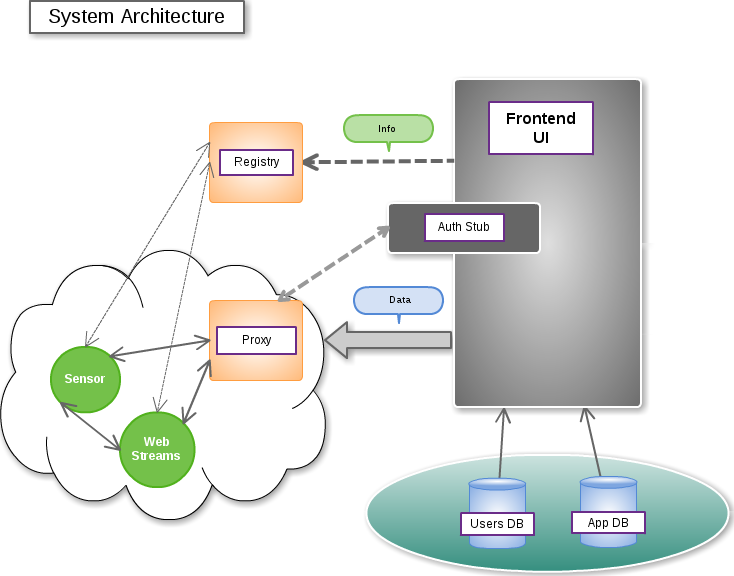
\includegraphics[scale=0.5]{images/Structure.png}   
\caption[System Architecture]{System Architecture}
\label{img:structure}                           
\end{figure}

\subsection{Functional Requirements}
\begin{figure}[!ht]
\centering
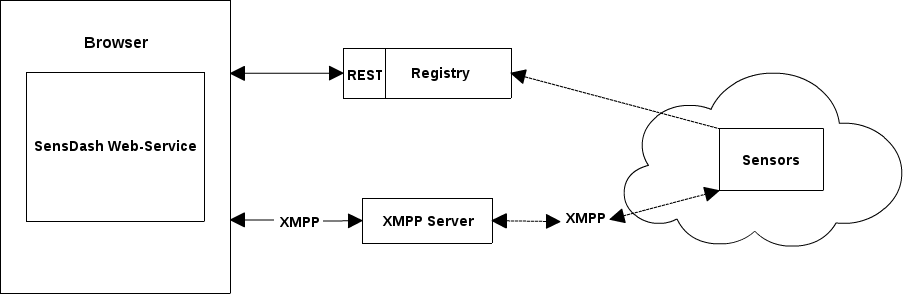
\includegraphics[scale=0.5]{images/Interface.png}   
\caption[Interface]{Interface}
\label{img:interfaces}                           
\end{figure}

\section{Data Tier}
   As was mentioned in section 4.1 Data Tier consists source of data that have to be retrieved by application tier to a client tier. Where is source of data is a data provided by sensors, in a specific type by using specific protocol, that will be nadled by Application Tier. The main focuse of this section determine possible characteristics of streamed data that can be retrieved by Client Tier in a lightweight scenario for mobile devices.
   \newline
    Streaming media is multimedia that is constantly received by and presented to an end-user while being delivered by a provider. Its verb form, "to stream", refers to the process of delivering media in this manner; the term refers to the delivery method of the medium rather than the medium itself. In general, media files can be delivered in one of three ways, via streaming, progressive download, or adaptive bitrate streaming.  Each has its purpose.
  \newline
    Streaming involves delivering the media to the client via a server process using specific streaming protocols (such as XMPP).  Video playing begins almost immediately, especially if the video file was encoded at a data rate similar to the effective bandwidth of the target viewer.  Streaming video is also often not cached by the client so a local copy of the video is not held in its entirety on the client machine.  While it is not impossible for an enterprising person to capture and hold a copy of the stream, it takes more effort than the casual viewer may be willing to take on.  To adapt for the slowest common denominator in regard to end-user bandwidth, streaming videos are often encoded at lower quality and data rates.
  \newline
    Progressive download simply delivers a media file via traditional webserver technologies.  The file begins playing on the client as soon as enough data has been buffered to provide a smooth uninterrupted viewing experience.  Progressive downloaded files are easier to capture since an entire copy of the file is downloaded to the local device.  Also, the quality of the file can be higher simply because a user on a slower connection will just have to wait longer for the viewing to begin.
  \newline
    Adaptive bitrate streaming is a kind of best of both worlds.  As the name implies, adaptive bitrate is a streaming technology and generally requires a dedicated streaming server.  In this case, media files are transcoded into multiple bitrates with the appropriate streaming being delivered to the user based on their available bandwidth.  Adaptive streaming servers can also dynamically change the bitrate as network conditions dictate\cite{ilias2013study}.
  \newline
  This explanation shows that adaptive bitrate streaming is the most valuable and suitable for concept of a generic frontend.
  But it is necessary to go deeply in details to define limits and understanding of "good quality", "bad quality", "excellent quality".
  All three delivery methods are forms of Adaptive Bit Rate Streaming. This delivery method will have a massive impact on every aspect of Internet video delivery because it allows the stream to actually adapt the video experience to the quality of the network and the device's CPU.
  \newline
  In other words, the video stream can increase or decrease the bit rate and resolution of the video (its quality) in real time so that it’s always streaming the best possible quality the available network connection can support. The better the network connection, the better the video image quality. The fact that the stream handles all of this complexity means the mobile video viewer doesn’t have to do anything; everything is left to the stream and the player.
  \newline
  So how does this all work? To prep your video content for HLS, you start off with a high quality version of your video and encode multiple copies of it using MPEG-4 H.264. These copies are at various bit rates and resolutions ranging from lower quality renditions appropriate for slower 3G connections, up to extremely high quality renditions suitable for fast devices on fast networks. The renditions are then wrapped into MPEG-2 Transport Streams and chopped up into 10 second segments or chunks. It’s these segments that are eventually streamed to an HTML5 Video Player on a mobile device, browser or set-top box, and because the player receives the video in 10 second chunks and can detect the quality of the network connection, it can switch to a higher or lower quality video segment every ten seconds if bandwidth conditions change.
  \newline
  Mobile platform such as iOS/Mobile Encoding supports at least two video types: 3GP + MPEG-4 for less sophisticated devices, and H.264 + MP4 for smartphones. One output video can cover all of smartphone users – iPhone/iPad/iPod, Android, and (for the most part) Blackberry too. Toss in PSP, PS3, and Xbox 360 for good measure. Mobile devices well using a handful of standard encoding profiles. Start with the Universal Smartphone Profile for wide compatibility; add in an Advanced Smartphone Profile version for the more advanced devices; and round out mobile list with a legacy profile for widest compatibility – either our Legacy Smartphone Profile (below), or even a 3GP video for even wider compatibility. The following defaults are the starting point for these profiles. Default these settings by default, but you can replicate them easily enough in whatever encoding tool you're using. Defaults: Video: H.264, Level 3.0, Baseline profile Audio: AAC, 1-2 channels
  %- data on demand%
  %Your model of data streams should consider that some streams can be replayed
%and some cannot because they contain live data. Also, some may be adaptive,

\subsection{Sensor Registry}
\subsection{Proxy}
\subsection{Authentification Stub}
\subsection{Databases}

\section{Summary}
In this master thesis, a first web-based prototype (portal) for such services is to be
created. Along with it, a light-weight scenario service registry will be needed. Users
should be able to explore not just services, but also the information provided by
them, and eventually be led to advanced usage patterns such as the development
of third-party applications to access the information data and real-time streams.
When dealing with videos, delivering the best possible video experience is the ultimate goal for every web team.  We all have seen good evidence that several HTML5 compliant video players (VideoJS, HTML5Video, JW Player, etc.) are becoming excellent alternatives when a fallback for non-flash support is required.  Perhaps the answer for the title/question of this article “is HTML5 the real fix for videos?” remains unanswered; but the hybrid solutions (Flash and HTML5) can be good examples of how to deliver video content, regardless of which device or browser users are using. After all, users do not necessarily care about how their videos are being delivered or processed. 